\documentclass[aspectratio=169,11pt]{beamer}
\usepackage[T1]{fontenc}
\usepackage[utf8]{inputenc}
\usepackage[brazil]{babel}
\usepackage{lmodern}
\usepackage{booktabs,tabularx,array}
\usepackage{amsmath,amssymb}
\graphicspath{{../projeto/figs/}}

% ---------------------------------------------------------------- estilo
\definecolor{azul}{HTML}{1F5FA8}
\definecolor{roxo}{HTML}{7B3FA0}
\definecolor{laranja}{HTML}{D07A1C}
\definecolor{cinza}{HTML}{5A5A5A}
\definecolor{fundo}{HTML}{F3F6FA}
\setbeamertemplate{navigation symbols}{}
\setbeamercolor{frametitle}{fg=azul,bg=white}
\setbeamerfont{frametitle}{series=\bfseries,size=\Large}
\setbeamertemplate{frametitle}{\vspace{0.35cm}\insertframetitle\par\vspace{0.05cm}{\color{azul}\rule{\linewidth}{0.8pt}}}
\setbeamercolor{normal text}{fg=black!85}
\setbeamercolor{structure}{fg=azul}
\setbeamertemplate{itemize item}{\color{azul}$\blacktriangleright$}
\setbeamertemplate{itemize subitem}{\color{cinza}\textendash}
\setbeamercolor{block title}{fg=white,bg=azul}
\setbeamercolor{block body}{bg=fundo}
\setbeamertemplate{blocks}[rounded][shadow=false]
\setbeamertemplate{footline}{%
  \leavevmode\hbox to\paperwidth{\hspace{0.4cm}{\color{cinza}\tiny Benchmarking do YOLOX-Nano int8 em MCU e SBC}\hfill
  {\color{cinza}\tiny\insertframenumber/\inserttotalframenumber}\hspace{0.4cm}}\vspace{0.25cm}}
\newcommand{\mcu}{\textcolor{roxo}{\textbf{MCU}}}
\newcommand{\sbc}{\textcolor{azul}{\textbf{SBC}}}
\newcommand{\destaque}[1]{\textcolor{azul}{\textbf{#1}}}
\newcolumntype{L}{>{\raggedright\arraybackslash}X}

\title{Benchmarking de Inferência do YOLO Quantizado em MCU e SBC}
\subtitle{Desempenho e eficiência energética do YOLOX-Nano para detecção de EPIs em \emph{Edge AI}}
\author{Filipe Matias \and Guilherme Lucas\\[2pt]{\small Orientador: Prof. Herbert Oliveira Rocha}}
\institute{\small PPCA, Universidade Federal de Roraima\\Arquitetura e Organização de Computadores}
\date{\small Novembro de 2026}

\begin{document}

% 1 ----------------------------------------------------------------
{\setbeamertemplate{footline}{}
\begin{frame}
\vspace{0.6cm}
{\color{azul}\LARGE\bfseries \inserttitle\par}
\vspace{0.2cm}
{\large \insertsubtitle\par}
\vspace{0.3cm}
{\color{azul}\rule{\linewidth}{0.8pt}}
\vspace{0.4cm}

\insertauthor\par
\vspace{0.3cm}
{\color{cinza}\insertinstitute\par\vspace{0.1cm}\insertdate\par\vspace{0.2cm}\small Código, dados e artigo: github.com/GuilhermeBn198/ptt6-yolox-edge-bench}
\end{frame}}

% 2 ----------------------------------------------------------------
\begin{frame}{Motivação}
\begin{columns}[T]
\column{0.55\textwidth}
\begin{itemize}
\item Inferência na borda reduz latência, tráfego e exposição de dados, mas é limitada por memória, computação e energia.
\item Dois extremos:
  \begin{itemize}
  \item \mcu: consumo baixo, memória de KB a poucos MB;
  \item \sbc: Linux completo, mais desempenho, mais consumo.
  \end{itemize}
\item Monitoramento de EPIs em canteiros: inspeção por longos períodos, muitas vezes com energia restrita.
\end{itemize}
\column{0.42\textwidth}
\begin{block}{Lacuna}
Faltam comparações diretas e reprodutíveis do \emph{mesmo} detector quantizado nas duas classes de plataforma, com
acurácia, latência e energia avaliadas em conjunto.
\end{block}
\end{columns}
\end{frame}

% 3 ----------------------------------------------------------------
\begin{frame}{Pergunta de pesquisa e hipóteses}
\begin{block}{Pergunta}
Como se comparam latência, throughput e energia por inferência entre o ESP32-S3 e o Raspberry Pi Zero 2 W ao
executar o mesmo YOLOX-Nano int8, com a acurácia como condição de validade?
\end{block}
\vspace{0.2cm}
\begin{itemize}
\item \destaque{H1}: o \sbc\ tem throughput maior, mas energia por inferência igual ou superior (consumo estático mais alto).
\item \destaque{H0}: não há diferença de throughput nem de energia.
\item \destaque{H2}: no \sbc, o int8 reduz latência e energia em relação ao fp32, ao custo de uma perda de acurácia quantificada.
\end{itemize}
\vspace{0.1cm}
{\small\color{cinza} Critério de validade: retenção $\rho=\mathrm{mAP}_{int8}/\mathrm{mAP}_{fp32}\geq0{,}99$ (referência do MLPerf).}
\end{frame}

% 4 ----------------------------------------------------------------
\begin{frame}{Plataformas, modelo e dados}
\small
\begin{tabularx}{\linewidth}{lLL}\toprule
 & \textcolor{roxo}{\textbf{MCU: ESP32-S3}} & \textcolor{azul}{\textbf{SBC: Raspberry Pi Zero 2 W}}\\\midrule
CPU & Xtensa LX7, 240\,MHz, SIMD de 128 bits & Cortex-A53, 4 núcleos, 1\,GHz, NEON\\
Memória & 512\,KB SRAM $+$ 8\,MB PSRAM octal & 512\,MB LPDDR2\\
Runtime & esp-tflite-micro $+$ ESP-NN, 1 núcleo & ai-edge-litert $+$ XNNPACK, 1/2/4 threads\\\bottomrule
\end{tabularx}
\vspace{0.3cm}
\begin{columns}[T]
\column{0.5\textwidth}
\begin{itemize}
\item \destaque{Modelo}: YOLOX-Nano (0,91\,M parâmetros), ajuste fino a $416\times416$.
\item \destaque{Mesmo arquivo int8} nas duas placas (1,16\,MiB, hash registrado); fp32 como referência no \sbc.
\end{itemize}
\column{0.47\textwidth}
\begin{itemize}
\item \destaque{Dados}: Construction-PPE, 11 classes; classe principal: colete.
\item 50 imagens de teste convertidas em tensores brutos idênticos byte a byte.
\end{itemize}
\end{columns}
\end{frame}

% 5 ----------------------------------------------------------------
\begin{frame}{Metodologia}
\begin{columns}[T]
\column{0.5\textwidth}
\textbf{Janela medida} (relógios monotônicos)\\[2pt]
\centerline{$t_{total}=t_{pre}+t_{inf}+t_{post}$}
\vspace{0.15cm}
\begin{itemize}\small
\item Imagem já em memória; transferência pela serial fica fora da janela.
\item Sem E/S dentro da janela.
\item 3 blocos de 10 inferências válidas ($n=30$), aquecimento descartado.
\item Mann-Whitney, $\delta$ de Cliff, IC por \emph{bootstrap} BCa.
\end{itemize}
\column{0.47\textwidth}
\small
\begin{tabularx}{\linewidth}{lL}\toprule
E0 & Acurácia fp32 $\times$ int8 (mAP)\\
E1 & Equivalência das saídas entre runtimes\\
E2 & Piloto: aquecimento e repetições\\
E3 & Latência por fase (int8 e fp32)\\
E3b & Escala com 1, 2 e 4 threads\\
E4 & 60\,s contínuos e deriva térmica\\
E5 & Memória, energia, \emph{break-even}, energia por ciclo\\\bottomrule
\end{tabularx}
\end{columns}
\end{frame}

% 6 ----------------------------------------------------------------
\begin{frame}{Modelo de energia (estimado, sem medição física)}
\begin{columns}[T]
\column{0.56\textwidth}
\footnotesize
$E=P_{pre}\,t_{pre}+P_{inf}\,t_{inf}+P_{post}\,t_{post}$\\[3pt]
Potência por modo, \destaque{na entrada de 5\,V de cada placa}:\\[3pt]
\begin{tabular}{llr}\toprule
Placa & Modo & Nominal [faixa] (W)\\\midrule
\sbc & ocioso & 0,60 [0,50; 1,00]\\
\sbc & 4 núcleos & 2,30 [1,85; 2,90]\\
\mcu & ativo & 0,44 [0,24; 0,54]\\
\mcu & ocioso & 0,24 [0,11; 0,24]\\
\mcu & acréscimo da placa & 0 [0; 0,25]\\\bottomrule
\end{tabular}
\column{0.40\textwidth}
\small
\begin{itemize}
\item \sbc: medições publicadas da placa.
\item \mcu: datasheet do ESP32-S3 (Tab.\ 5-9), regulador linear no nominal.
\item Conclusões testadas nos extremos.
\item Por ciclo de inspeção:\\[2pt]
$E_{ciclo}(f)=E+P_{ocioso}\,(1/f-t_{total})$
\end{itemize}
\end{columns}
\end{frame}

% 7 ----------------------------------------------------------------
\begin{frame}{E0: o artefato int8 não atinge o critério de acurácia}
\begin{columns}[T]
\column{0.56\textwidth}
\small
\begin{tabular}{lrrr}\toprule
Modelo & mAP@50 & mAP@50:95 & AP@50 colete\\\midrule
fp32 & 55,0\% & 27,2\% & 88,8\%\\
int8 & 16,7\% & 6,4\% & 47,1\%\\\midrule
$\rho$ & \textcolor{azul}{0,30} & 0,23 & 0,53\\\bottomrule
\end{tabular}\\[3pt]
{\scriptsize\color{cinza} Teste: 141 imagens, 1.251 anotações; IC 95\% de $\rho$: 0,26 a 0,34.}
\column{0.41\textwidth}
\begin{itemize}\small
\item Retenção de 30\%, contra a meta de 99\%.
\item Calibração com 100 imagens em RGB, enquanto treino e inferência usam BGR.
\item \destaque{Consequência}: tempos e energias descrevem o custo do grafo int8, não um detector apto à operação.
\end{itemize}
\end{columns}
\end{frame}

% 8 ----------------------------------------------------------------
\begin{frame}{E1: o mesmo int8 dá saídas diferentes por runtime}
\small
\begin{tabular}{lrrr}\toprule
Comparação & Mesmas classes & Caixas com IoU $\geq0{,}95$ & IoU médio\\\midrule
PC LiteRT $\times$ \sbc\ LiteRT & 100\% & 97,3\% & 0,996\\
PC LiteRT $\times$ \mcu & 30\% & 1,7\% & 0,745\\
PC TFLM ref.\ $\times$ \mcu & 32\% & 0,9\% & 0,698\\\bottomrule
\end{tabular}
\vspace{0.3cm}
\begin{itemize}
\item Mesmo runtime (PC e Raspberry): saídas equivalentes.
\item Runtimes distintos (XNNPACK, TFLite Micro, ESP-NN): saídas numericamente diferentes.
\item \destaque{Qualidade agregada igual}: F1 de 0,32 e revocação de 0,21 nas quatro execuções (50 imagens, 448 objetos).
\end{itemize}
\end{frame}

% 9 ----------------------------------------------------------------
\begin{frame}{E3 e E3b: latência e escala com threads}
\centering
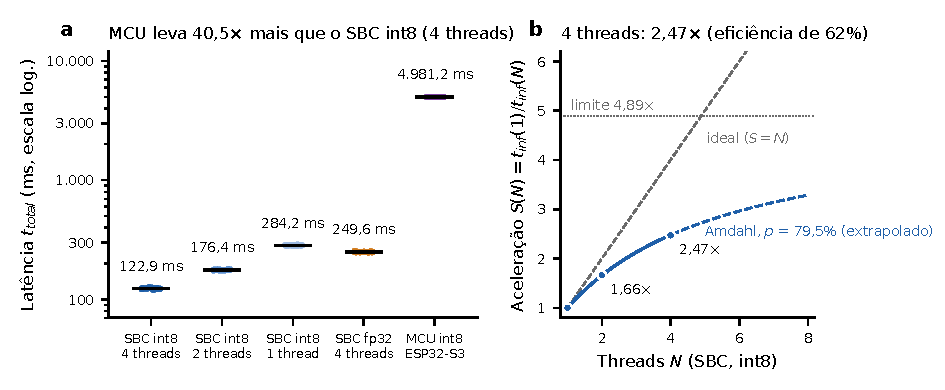
\includegraphics[width=0.93\linewidth]{fig_latencia.pdf}\\[-2pt]
\small
\sbc\ int8 (4 threads): \destaque{122,9\,ms} (8,1 inf/s) \quad
\mcu: \textcolor{roxo}{\textbf{4.981,2\,ms}} (0,20 inf/s) \quad
Amdahl: $p=79{,}5\%$
\end{frame}

% 10 ----------------------------------------------------------------
\begin{frame}{E5: energia por inferência}
\centering
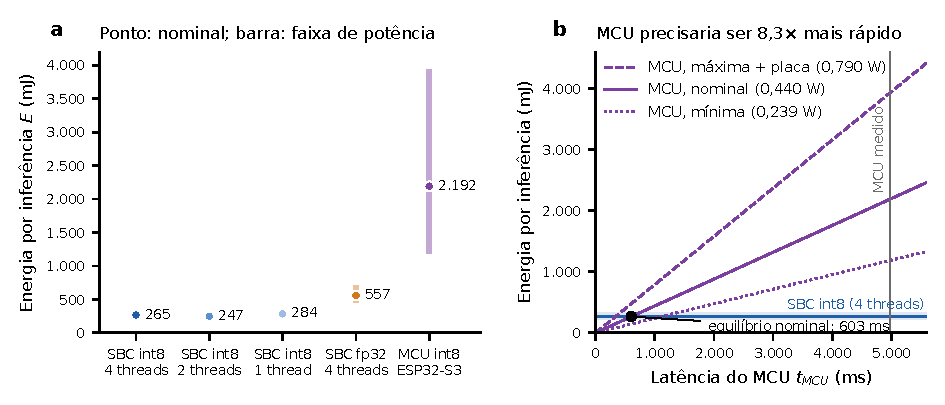
\includegraphics[width=0.93\linewidth]{fig_energia.pdf}\\[-2pt]
\small
\sbc: \destaque{265\,mJ} \quad \mcu: \textcolor{roxo}{\textbf{2.192\,mJ}} (8,3$\times$ mais) \quad
Nos extremos: de 3,6$\times$ a 18,5$\times$ mais no \mcu
\end{frame}

% 11 ----------------------------------------------------------------
\begin{frame}{E5: energia por ciclo de inspeção}
\centering
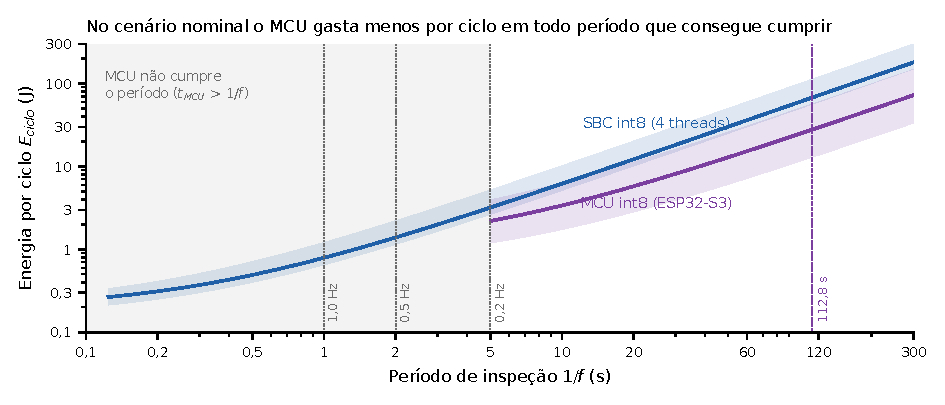
\includegraphics[width=0.93\linewidth]{fig_ciclo.pdf}\\[-2pt]
\small
A 0,2\,Hz: \mcu\ 2,20\,J, \sbc\ 3,19\,J \quad Uma por minuto: 2,4$\times$ \quad Pior caso: a partir de 113\,s
\end{frame}

% 12 ----------------------------------------------------------------
\begin{frame}{Teste das hipóteses}
\small
\begin{tabularx}{\linewidth}{lLl}\toprule
 & Resultado & Veredito\\\midrule
\textbf{H1}, throughput & \sbc\ 40,5$\times$ mais rápido ($p<10^{-10}$, $\delta=-1$) & \textcolor{azul}{\textbf{confirmada}}\\
\textbf{H1}, energia & \sbc\ gasta \emph{menos} por inferência em todos os cenários & \textcolor{laranja}{\textbf{não sustentada}}\\
\textbf{H0} & diferença nos dois desfechos (bilateral, $p<10^{-10}$) & \textcolor{laranja}{\textbf{rejeitada}}\\
\textbf{H2} & int8: $t_{inf}$ 2,16$\times$ e energia 2,10$\times$ menores; $\rho=0{,}30$ & \textcolor{azul}{\textbf{confirmada no custo}}\\\bottomrule
\end{tabularx}
\vspace{0.35cm}
\begin{block}{Por que H1 falha}
A diferença de tempo (40,5$\times$) supera de longe a diferença de potência média (4,9$\times$): o consumo estático do
\sbc\ não compensa quando a inferência é contínua.
\end{block}
\end{frame}

% 13 ----------------------------------------------------------------
\begin{frame}{Discussão: quando cada plataforma compensa}
\begin{columns}[T]
\column{0.48\textwidth}
\begin{block}{Inspeção acima de 0,2\,Hz}
Só o \sbc\ cumpre o período (o \mcu\ leva 4,98\,s por inferência), e ele também gasta menos por inferência.
\end{block}
\column{0.48\textwidth}
\begin{block}{Inspeção a cada 5\,s ou mais}
O \mcu\ gasta menos por ciclo no cenário nominal, porque o \sbc\ fica ocioso a 0,6\,W entre as imagens.
\end{block}
\end{columns}
\vspace{0.3cm}
\begin{itemize}\small
\item A escolha depende da \destaque{taxa de inspeção exigida} pela aplicação.
\item A vantagem por ciclo do \mcu\ é sensível ao acréscimo de potência da placa: some acima de 0,26\,W.
\item Gargalo do \mcu\ provavelmente fora da aritmética (PSRAM, flash, kernels de referência); sem perfilamento por operador, fica como hipótese.
\end{itemize}
\end{frame}

% 14 ----------------------------------------------------------------
\begin{frame}{Ameaças à validade}
\small
\begin{tabularx}{\linewidth}{LL}\toprule
Ameaça & Tratamento\\\midrule
Int8 abaixo do critério ($\rho=0{,}30$) & resultados de custo como custo do grafo\\
Energia estimada, não medida & mesmo escopo (5\,V) nas duas placas; cenários extremos\\
Potência do \sbc\ de medições publicadas & faixa ampla; consistente com o valor oficial (1,75\,W)\\
Plataforma confundida com runtime e linguagem & resultados descrevem o par dispositivo $+$ software\\
Um exemplar de cada placa & testes medem a repetibilidade da medição\\
Aquisição da imagem fora da janela & a 0,2\,Hz, a folga do \mcu\ é de só 19\,ms\\\bottomrule
\end{tabularx}
\end{frame}

% 15 ----------------------------------------------------------------
\begin{frame}{Conclusão e próximos passos}
\begin{itemize}
\item O Raspberry Pi Zero 2 W foi \destaque{40,5$\times$ mais rápido}, e o ESP32-S3 gastou \destaque{8,3$\times$ mais energia por inferência}: H1 não se sustenta.
\item Em inspeção periódica e espaçada, o ESP32-S3 \destaque{gasta menos por ciclo} (o SBC gasta 1,45$\times$ mais a 5\,s e 2,4$\times$ a 60\,s), mas a conclusão depende da potência real da placa.
\item No \sbc, o int8 cortou latência e energia pela metade em relação ao fp32.
\end{itemize}
\vspace{0.15cm}
\begin{block}{Próximos passos}
\begin{itemize}\small
\item Recalibrar o int8 na ordem de canais do treino (ou adotar outra versão quantizada do YOLO) e repetir as medições.
\item Perfilar a inferência por operador no ESP32-S3.
\item Medir a potência das placas quando houver instrumentação.
\end{itemize}
\end{block}
\end{frame}

\end{document}
